\subsection{A Historia}\label{history}


Toru Iwatani, criador do jogo PAC-MAN, se inspirou em uma história infantil sobre uma criatura que protegia as crianças dos monstros por comê-los. Um dos métodos de design Iwatani incluído a palavras-chave associadas com uma história para auxiliar no desenvolvimento de suas ideias. O kanji da palavra taberu ("comer"), tornou-se a premissa para o jogo. A palavra kuchi ("boca") tem um formato quadrado para seu símbolo kanji e forneceu a inspiração para o jogo da principal lenda personagem-o mais conhecido de Iwatani receber sua inspiração de uma pizza com uma fatia faltando foi, por sua própria admissão, não inteiramente correta: 

\begin{quote}
	\textit{"Bem, é uma meia verdade. Em caráter do japonês para boca (Kuchi) tem uma forma quadrada. Não é circular como a pizza, mas eu decidi arredonda-lo. Havia a tentação de fazer a forma de Pac-Man menos simples. Enquanto eu estava projetando este jogo, alguém sugeriu adicionar os olhos. Mas nós finalmente descartamos essa ideia, porque uma vez que nós adicionássemos os olhos, nós gostaríamos de adicionar óculos e talvez um bigode. Não teria fim. O alimento é a outra parte do conceito básico. Na minha concepção inicial, eu tinha colocado o jogador em meio a comida por toda a tela. Então eu pensei sobre isso, percebi que o jogador não saberia exatamente o que fazer: o objetivo do jogo seria obscuro. Então, eu criei um labirinto e coloquei a comida nele. Assim, quem jogasse o jogo teria alguma estrutura ao se mover através do labirinto. Os japoneses têm uma gíria - paku-paku - eles usam para descrever o movimento da boca abrindo e fechando, enquanto se come. O nome Puck-Man veio essa palavra. "}

- Toru Iwatani
\end{quote}

Os monstros da história das crianças foram incluídos como quatro fantasmas que perseguem o jogador através do labirinto, proporcionando um elemento de tensão. Ataques contra o jogador foram projetados para vir em ondas (semelhante ao \textbf{Space Invaders}), em oposição a um ataque sem fim, e cada fantasma foi dada uma personalidade única e caráter. A história das crianças também incluiu o conceito de kokoro ("espírito") ou uma força de vida utilizada pela criatura que lhe permitia comer os monstros. Toru incorporou este aspecto da história de quatro pastilhas de energia comestíveis no labirinto para virar a mesa contra os fantasmas, tornando-os vulneráveis ​​a ser comido pelo jogador.

A aparência de Puck-Man continuou a evoluir por mais de um ano. Uma grande quantidade de tempo e esforço foi feito para desenvolver os fantasmas padrões de movimentos únicos através do labirinto e aprimorando as variáveis ​​do jogo de dificuldade, como placas foram apuradas. Símbolos de bônus (incluindo o carro-chefe Galaxian) foram adicionados à mistura, em algum momento, e os fantasmas foram finalmente nomeados: Akabei, Pinky, Aosuke, e Guzuta. Efeitos sonoros e música foram alguns dos toques finais adicionados, com o desenvolvimento se aproximando do fim, eram feitos ajustes constante do comportamento dos fantasmas. Tornando-se por fim como apresentado na figura \ref{pac1}.

\end{multicols}
\begin{figure}[h]
\begin{center}
  \centering
  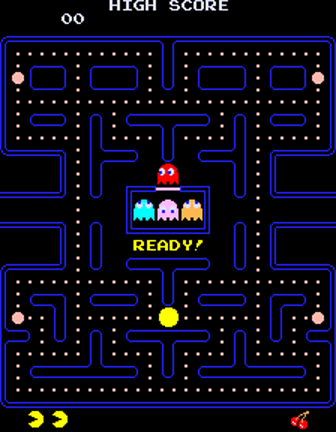
\includegraphics[scale=0.45]{./fts/lvl1}
  \caption{Pac-Man.\\O clássico dos anos 80 só foi ter um score perfeito - máximo de pontos, sem falhas ou mortes - em 1999, quando \textit{Billy Mitchell} consegui a incrível marca de $3,333,360$ pontos, após vencer os consecutivos 256 leveis do jogo.}
  \label{pac1}
\end{center}
\end{figure}
\begin{multicols}{2}

Midway era uma distribuidora de jogos que funcionam com moedas nos EUA. Estavam sempre procurando o próximo grande sucesso do Japão para licenciar e trazer para a América. Eles optaram por tanto Puck-Man e Galaxian, modificando os armários e obras de arte para torná-los mais fáceis de fabricar, bem como proporcionar um olhar mais americano.

Puck-Man passou por grandes mudanças: o gabinete foi ligeiramente modificado, mudando a cor de branco para um amarelo brilhante para fazê-lo sobressair no arcade. O detalhado gabinete multi-colorido foi substituído com mais barato, para produzir em três cores de arte que ilustra uma representação icônica de Puck-Man (agora desenhado com olhos e pés) e um fantasma azul. Nomes ingleses foram dadas para os fantasmas (Blinky, Pinky, Inky e Clyde), e o título foi mudado da Namco para  a Midway. A mudança mais significativa para Puck-Man foi o nome. A Midway temia que seria muito fácil para vândalos desagradável de espírito para mudar o P em Puck-Man para um F, criando um epíteto desagradável. Não querendo seu produto associado a esta palavra, a Midway renomeou o jogo para Pac-Man antes de liberá-lo para os arcades americanos em outubro de 1980.\cite{dossier}

\subsection{Os fantasmas e seus comportamentos}\label{desafios}

Ao final da implementação do jogo original, os fantasmas ganharam características e personalidades, possuindo cada um uma AI distinta. Essa é provavelmente uma das ultimas implementações que será realizada neste nosso jogo - se vier a ser implementada. No jogo original, haviam apenas quatro fantasmas, dos quais falaremos um pouco mais sobre eles.

\subsubsection{Blinky}\label{blinky}

O fantasma vermelho é apropriadamente descrito como o de uma sombra e é mais conhecido como "Blinky". No Japão, seu personagem é representado pelo oikake palavra, que significa "correr para baixo ou prosseguir". Blinky parece ser sempre o primeiro dos fantasmas para acompanhar o Pac-Man no labirinto. Ele é de longe o mais agressivo dos quatro e vai obstinadamente buscar Pac-Man uma vez atrás dele.

Todos os fantasmas movem-se com a mesma taxa de velocidade quando se inicia um nível, mas Blinky irá aumentar a sua taxa de velocidade duas vezes por nível baseado no número de pontos que permanecem no labirinto. Enquanto neste estado acelerado, Blinky é comumente chamado de \textit{"Cruise Elroy"}, mas ninguém parece saber onde esse costume se originou ou o que significa. No primeiro nível, por exemplo, Blinky torna-se Elroy quando existem 20 pontos remanescentes no labirinto, vindo a ser tão rápido como Pac-Man.\cite{dossier}

\subsubsection{Pinky}\label{pinky}

Apelidado de "Pinky", o fantasma rosa é descrito como alguém que é rápido. No Japão, ele é caracterizado como machibuse, que significa "para realizar uma emboscada", talvez porque Pinky sempre parece ser capaz de chegar à frente de você e pega-lo quando você menos espera. Ele se move sempre à mesma velocidade como Inky e Clyde, no entanto, o que sugere que "rápido" é uma má tradução do machibuse . Pinky e Blinky muitas vezes parecem estar trabalhando em conjunto para encurralar Pac-Man, deixando-o sem ter para onde correr.\cite{dossier}

No modo perseguição, Pinky se comporta assim, porque ele não tem como alvo o Pac-Man diretamente. Em vez disso, ele seleciona um deslocamento quatro peças adiante de Pac-Man na direção em que Pac-Man está se movimentando. Porém o jogo original carregava um bug. Se o Pac-Man estivesse se movimentando para cima, Pinky não apenas quatro posições para cima, mas também quatro posições para a esquerda, mirando assim a uma distancia de $\sqrt{32}$ posições na diagonal superior esquerda de Pac-Man. Este bug ocorre devido a um problema de overflow, como pode ser observado no trexo abaixo onde a rotina de  busca de Pinky é transcrita.

\begin{lstlisting}[language=MSP430,title=\textit{Subrotina de alvo de Pinky \cite{pinkybug}},numbers=none]
; load DE with Pac-man's position
278E ED5B394D 	LD  DE,(#4D39) 	
; load HL with Pac-man's direction vector
2792 2A1C4D 	LD  HL,(#4D1C)	
; double Pac-man's direction vector
2795 29 		ADD HL, HL		
; quadruple Pac-man's direction vector
2796 29 		ADD HL, HL		
; add result to Pac-Man's position to give target
2797 19 		ADD HL, DE 		
\end{lstlisting}

Em todas as demais direções, o vetor do Pac-man possui apenas uma coordenada não nula, porém quando quando esta subindo, este vetor recebe o valor $(1,-1)$, assim, HL passa a ter como valor final um vetor de valor $(4,-4)$.

\subsubsection{Inky}\label{inky}

 O fantasma azul é apelidado de "Inky" e seu personagem é descrito como alguém que é tímido. No Japão, ele é retratado como Kimagure, que significa "um temperamento inconstante, temperamental, ou irregular". Talvez não surpreendentemente, Inky é o menos previsível dos fantasmas. Às vezes, ele persegue agressivamente Pac-Man como Blinky, outras vezes ele salta à frente de Pac-Man como Pinky faria. Ele pode até mesmo vagar como Clyde na ocasião! Na verdade, Inky pode ser o fantasma mais perigoso de todos, devido ao seu comportamento errático.\cite{dossier}
 
 \subsubsection{Clyde}\label{clyde}
 
 O fantasma laranjado é apelidado de "Clyde" e é caracterizado como aquele que é chato. No Japão, seu personagem é descrito como otoboke, ou seja, "ignorância fingindo", e seu apelido é "Guzuta", que significa "aquele que fica para trás". Na realidade, Clyde se move na mesma velocidade que Inky e Pinky, então sua descrição do personagem é um pouco erronea. Clyde é o fantasma último a deixar a caneta (local onde os fantasmas começam) e tende a separar-se dos outros fantasmas por se afastando do Pac-Man e fazer sua própria lógica, quando ele não está patrulhando seu canto do labirinto. Apesar de não ser tão perigosos quanto os outros três fantasmas, o seu comportamento pode parecer imprevisível, e ainda deve ser considerado uma ameaça.
 
 
Durante o modo perseguição, Clyde muda sua lógica com base em sua proximidade com Pac-Man. Ele primeiro calcula a distância euclidiana entre sua posição e a de Pac-Man. Se a distância entre eles é de oito peças ou mais, Clyde busca Pac-Man diretamente como Blinky faz. Se a distância entre eles é inferior a oito peças, no entanto, Clyde muda seu comportamento para a forma que ele normalmente usa durante o modo de dispersão e vai para seu canto até que ele estar longe o suficiente para começar a busca por Pac-Man de novo.\cite{dossier}
